Several steps have been followed in order to enable the acquisition of meaningful data during the subjective tests. Theses steps included defining the test environment, choosing a rating framework and creating additional question that may help inferring informations about the participants and their way of rating content.

\subsubsection{Test Environment}
In order to make the results of our research reproducible the ITU P.910 recommendation \cite{rec1998p} have been followed. 
The parameters include aspects such as viewing distance, peak luminance of the screen or background room illumination.
As performing tests following these specifications is common at the Technical University of Ilmenau, a room meeting these requirements was available and therefore used.
The specifications of the room was the following for each of the parameters:


	
\subsubsection{Rating Framework}
The testing procedure which seems more suited to the case was Absolute Category Rating (ACR) \cite{rec1998p}, where different versions of an original sequence are shown to a test participant. 

For each sequence the participant issues categorical ratings from any of these 5 answers: \{Excellent, Good, Fair, Poor, Bad\}


The steps performed by a participants during a rating session can be seen in the figure \ref{fig:workflow:state_machine}.

\begin{figure}[h]
	\centering
	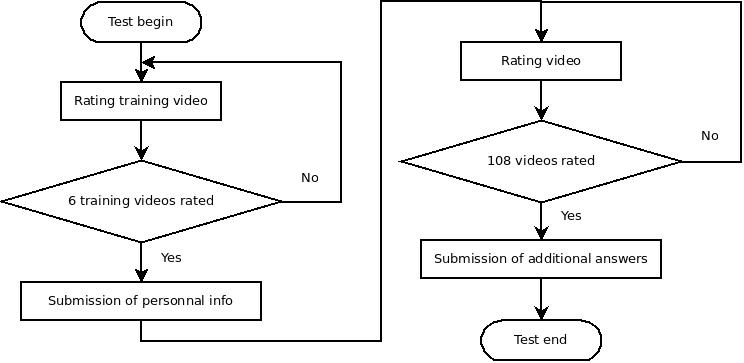
\includegraphics[width=3.5in]{rating_workflow}
	\caption{Detailed steps of the rating workflow}
	\label{fig:workflow:state_machine}
\end{figure}

\subsubsection{Additional collected data}
In order to gain more knowledge about the users behaviour, additional data is collected from the participants.

One of the suggestions of the ITU recommendation paper being the usage of several test questions in addition to the ratings \cite{rec1998p}, the following questions have been asked at the end of each rating session:

\begin{itemize}
	\item Presence of blocky artefacts
	\item Visible bands of colour
	\item Smoothness of the playback
	\item Have you seen 4K content before?
	\item Have you seen content on a 4k screen before?
	\item How sure were you about the rating that you provided?
\end{itemize}




These idea behind these question is dual as these questions may translate how users percieve/are sensitive to video features as well as how users may clearly express their perceptions. As it has already been noticed in previous experiments and in discussions with test participants: users may still rate using a different scales, thus spreading the final MOS or falsely being classified as outlier when their ratings may only represent a shift from the overall population. 

Moreover, mouse interactions have been collected during the rating of each sequence. The intent behind this is that as the MOS scale doesn't allow detailed answers some participants may hesitate between two answers and change their answers or hover with their mouse around some answers. Also, answering speed, which could be an indicator of a participant skipping answers or to the contrary being strongly confident of his answers. We believe that several informations can be extracted from these kind of behaviours:
\begin{itemize}
	\item Confidence in the participant sequence rating
	\item Confidence in the participant overall rating
	\item Intermediate scores (eg: 4.5)
\end{itemize}
